\chapter{Ferramentas e Metodologias Utilizadas}

Obviamente, assim como todas as outras aplicações web, foi utilizado o protocolo HTTP para comunicação entre cliente e servidor. Essa comunicação se inicia quando o cliente (no caso, o navegador do usuário) realiza uma requisição HTTP. Ao receber a requisição, o servidor web a processa, gera uma resposta pertinente e a devolve ao cliente~\cite{wikipediahttp}.

O código de aplicações web é dividido em duas principais categorias: o \textit{frontend}, responsável pela interação com o usuário, e o \textit{backend}, responsável por todo o processamento realizado no servidor. A compreensão desta distinção é essencial, pois existem linguagens e metodologias específicas, tanto para o desenvolvimento de cada uma delas, como para o planejamento da comunicação entre esses dois mundos. Mais adiante, as duas categorias serão explicadas em mais detalhes.

\section{RESTful}

O protocolo HTTP foi desenvolvido em paralelo com a arquitetura REST (Representational State Transfer),
\abbrev{REST}{Representational State Transfer}
que serve de molde para o desenvolvimento de aplicativos web, pois ilustra como eles devem se comportar~\cite{restthesis}. Uma aplicação que é desenvolvida segundo a arquitetura REST, é dita RESTful. Seguindo esta arquitetura no desenvolvimento da aplicação, uma série de vantagens são obtidas, como uma melhora na escalabilidade da mesma. Isto ocorre pois esta arquitetura segue uma lógica \textit{stateless}, isto é, o servidor não armazena estados, sendo necessária a transmissão de todas as informações inerentes ao processamento das requisições por meio das mesmas.

Para que a aplicação seja RESTful, devemos nos preocupar com alguns detalhes. É importante que cada recurso seja representado por uma única URI (Uniform Resource Identifier),
\abbrev{URI}{Uniform Resource Identifier}
mas para que isso seja possível, é necessário explorar ao máximo os seus métodos. Como a maioria dos recursos precisam ser relacionados a cada uma das ações do CRUD (Create, Retrive, Update, Destroy),
\abbrev{CRUD}{Create, Retrive, Update, Destroy}
é interessante que tais ações sejam relacionadas diretamente com os métodos do protocolo HTTP, visando manter inviolável a relação entre a URI e o recurso. Sendo assim, os quatro principais métodos do protocolo HTTP, que serão invocados no \textit{frontend}, devem ser relacionados aos quatro métodos do CRUD, que serão invocados no \textit{backend}. Em geral essa relação ocorre da seguinte forma:
\begin{itemize}
\item C (Create) - método POST
\item R (Retrive) - método GET
\item U (Update) - método PUT
\item D (Destroy) - método DELETE
\end{itemize}

\section{\textit{Frontend}}

O \textit{frontend} da aplicação é todo o código encarregado de realizar a interação com o usuário. No caso, trata-se de tudo que será enviado ao navegador. Esse código tem a finalidade de exibir de forma inteligível e interessante o resultado da requisição tratada pelo \textit{backend}, além de lidar com as entradas de dados (\textit{inputs}) do usuário. Para a construção do \textit{frontend} utilizamos algumas linguagens e bibliotecas, que serão elucidadas a seguir.

\subsection{HTML}

O HTML é a linguagem base do \textit{frontend}, pois as demais operam sobre seus elementos. Ela torna possível a interpretação das páginas web pelos navegadores. Esta linguagem sofreu algumas atualizações, porém, após mais de dez anos sem novas versões, ficou bastante defasada. Com os avanços da Internet, passaram a ser utilizados inúmeros \textit{plug-ins} para que páginas web fossem capazes de realizar algumas atividades essenciais, como reprodução de vídeos ou de áudio.

Esse atraso se prolongou até 2008, quando foi publicada uma nova versão, o HTML5, que ainda não esta completamente em vigor, porém cada vez mais em uso~\cite{wikipediahtml}. Essa nova versão dá suporte a diversas funcionalidades sem que sejam necessários \textit{plug-ins}. Dentre as funcionalidades implementadas estão a reprodução de vídeos , áudios, o \textit{drag and drop} e a exibição de imagens vetorizadas~\cite{videohtml}.

\subsection{CSS}

O CSS é uma linguagem criada para estilização de componentes HTML. Podemos dizer que os navegadores interpretam o CSS como adjetivos dos componentes HTML. É uma linguagem voltada para o ``como exibir'', enquanto o HTML se preocupa com ``o que exibir''. O CSS3, sua versão mais recente que trouxe diversas novas funcionalidades, vem sendo cada vez mais utilizado.

\subsection{Javascript}

O Javascript é uma linguagem de programação que, apesar de ser utilizada no desenvolvimento do \textit{frontend} da aplicação, se assemelha às linguagens de \textit{backend}, pela liberdade oferecida ao programador. É utilizada para dar interatividade às páginas web, visto que, apesar de essenciais, o HTML e o CSS não fornecem muita dinamicidade à mesma. Através da utilização de Javascript é possível alterar de forma livre o conjunto composto pelo HTML e CSS, mesmo após o carregamento completo da página. Inúmeras bibliotecas são construídas através da linguagem Javascript. Muitas delas também são utilizadas no \textit{frontend} de aplicações web, como a JQuery.

\subsection{AJAX (Asynchronous JavaScript and XML)}
\abbrev{AJAX}{Asynchronous JavaScript and XML}

O AJAX é um conjunto de técnicas que permite a criação de requisições assíncronas em páginas web. A sua utilização é interessante quando é necessária a troca de dados sem que seja preciso recarregar a página por inteiro. Resumidamente, uma implementação de AJAX é um trecho de código em Javascript, que faz com que seja realizada uma requisição XHR (XML HTTP Request),
\abbrev{XHR}{XML HTTP Request}
que será tratada e respondida pelo servidor. Essa resposta, que em geral é no formato XML (Extensible Markup Language)
\abbrev{XML}{Extensible Markup Language}
ou JSON (JavaScript Object Notation),
\abbrev{JSON}{JavaScript Object Notation}
é recebida pelo Javascript, podendo ser utilizada para atualizar elementos.

\subsection{JQuery}

A JQuery é talvez a biblioteca mais utilizada em Javascript no desenvolvimento de aplicações web. Diversas funcionalidades interessantes são implementadas por esta biblioteca, dentre elas, uma interface amigável para customização de requisições AJAX. É muito utilizada também para criar animações, como a inserção de elementos na tela de forma gradual.

\section{\textit{Backend}}

O \textit{backend} da aplicação é todo o código responsável pelo processamento da requisição até o momento da geração da resposta. Para exemplificar, pode-se pensar em uma requisição de abertura de sessão (\textit{login}) por meio da aplicação. Neste caso, o \textit{backend} é o código responsável por atividades como a verificação da existência do usuário ou a validação da senha inserida pelo mesmo. O \textit{backend} determina também qual o tipo da resposta que será devolvida ao usuário (falha ou sucesso na abertura de sessão, segundo o exemplo). Observando por outro prisma, o \textit{backend} pode ser encarado como o código responsável pela tomada de decisão.

O \textit{backend} pode ser implementado em inúmeras linguagens. Como é muito comum e recomendada a utilização de \textit{frameworks}, as linguagens relativas a estes acabam sendo as mais utilizadas. Linguagens como o SQL também são utilizadas no \textit{backend} da aplicação, já que o BD também o compõe.

Existem diversos \textit{frameworks} nas mais variadas linguagens, porém o escolhido para este trabalho foi o Ruby on Rails. A seguir serão explicados com detalhes os motivos da escolha, através de funcionalidades deste \textit{framework}.

\section{A escolha do Ruby on Rails}

O desenvolvimento ágil de aplicações web teve início com o surgimento do Ruby on Rails. Esta agilidade na implementação se deve a uma série de princípios adotados no desenvolvimento deste \textit{framework}, como o DRY (Don't Repeat Yourself) e o CoC (Convention over Configuration)~\cite{ieeecomparsionagileframeworks}. O DRY é um princípio de desenvolvimento de software que introduz a ideia de que uma mesma informação não deve ser repetida mais de uma vez ao longo do código. Este princípio simplifica o trabalho do desenvolvedor, evitando redundâncias e os problemas causados por elas. O CoC implica em adotar por padrão uma mesma configuração. Caso o desenvolvedor queira fugir do padrão, deve escrever código para isso, porém não deve escrever uma única linha para seguir os padrões.

Por ser pioneiro em desenvolvimento ágil de aplicações web, o Ruby on Rails teve o seu grande momento logo após o seu lançamento, e, por volta de 2006, atingiu o seu pico de interesse. Até hoje existe uma grande comunidade que o utiliza, porém, após o surgimento de diversos outros \textit{frameworks} para desenvolvimento ágil, ocorreu significativa queda no interesse. Estabilizou-se então dentre os \textit{frameworks} mais utilizados, como podemos notar através da figura~\ref{fig:curvainteresserails}, que indica a curva de interesse sobre os \textit{frameworks} ao longo dos anos.

\begin{figure}[H]
\centering
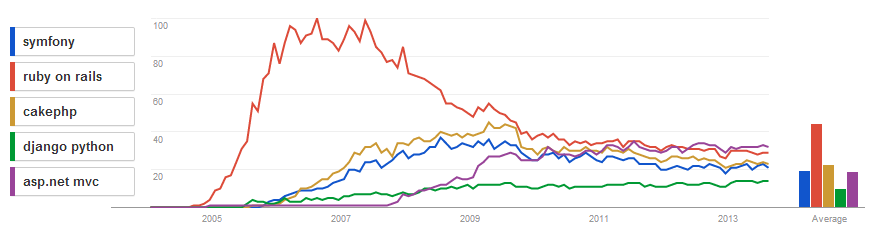
\includegraphics[width=0.8\textwidth]{figs/curva_de_interesse}
\caption[\textit{Curva de Interesse sobre os \textit{frameworks} ao longo dos anos}.]
{Curva de Interesse sobre os \textit{frameworks} ao longo dos anos~\cite{curvadeinteresseframeworks}.}
\label{fig:curvainteresserails}
\end{figure}

O Ruby on Rails é um \textit{framework} dito \textit{full-stack}, por ser utilizado obrigatoriamente por inteiro (ao contrário de outros \textit{frameworks}, onde seus módulos podem ser utilizados separadamente, como o Zend). Possui uma arquitetura MVC (Model-View-Controller),
\abbrev{MVC}{Model-View-Controller}
muito comum em diversos \textit{frameworks}, que será melhor detalhada a seguir. Esta arquitetura aplicada em um \textit{framework} \textit{full-stack} e aliada a conceitos como o DRY e o CoC, permite que em pouquíssimas linhas de código, enormes funcionalidades sejam implementadas, como veremos mais a frente.

\subsection{Arquitetura MVC}

Esta arquitetura realiza uma separação entre a parte que interage com o usuário (a visão) e a informação (o modelo), permitindo que esta seja acessada por meio de métodos em classes específicas (os controladores). Esta forma modularizada de desenvolvimento provê um excelente isolamento entre essas camadas com funções tão distintas, viabilizando a reutilização de código e tornando o mesmo mais legível, e, consequentemente, manutenível.

A figura ~\ref{fig:mvc} apresenta a arquitetura MVC aplicada ao \textit{framework} Ruby on Rails~\cite{basefiguramvc}. O servidor web repassa as requisições recebidas a um sistema de rotas, que é encarregado de enviá-las ao controlador correspondente. O sistema de rotas muitas vezes é definido no próprio servidor web, porém, o Rails possui sistema de rotas independente, como será elucidado na subseção ~\ref{subsec:sistrotas}. Os demais componentes, relativos ao MVC, serão melhor detalhados a seguir.

\begin{figure}[H]
\centering
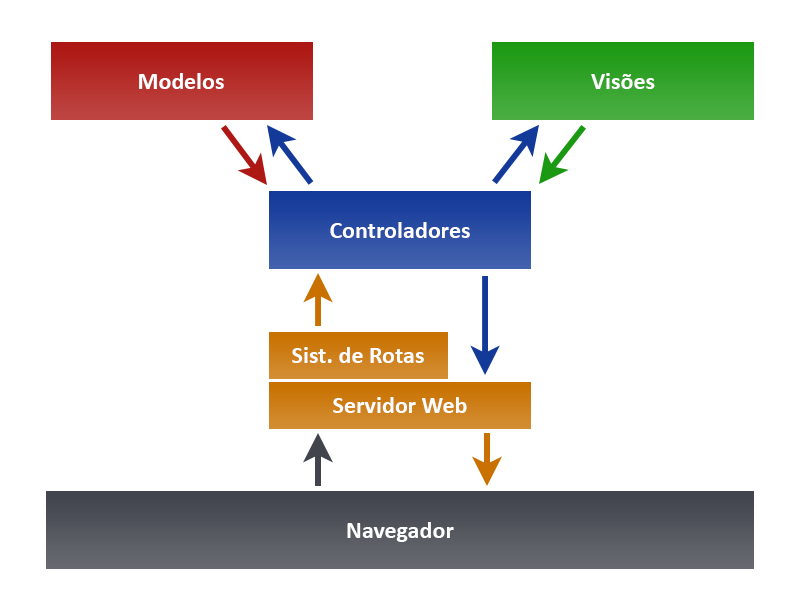
\includegraphics[width=0.8\textwidth]{figs/mvc}
\caption[\textit{Arquitetura MVC do \textit{framework} Ruby on Rails}.]
{Arquitetura MVC do \textit{framework} Ruby on Rails.}
\label{fig:mvc}
\end{figure}

\begin{itemize}

\item O Modelo

O modelo é o módulo responsável pela gerência do conhecimento da aplicação e sua manipulação segundo métodos específicos. Em geral, as aplicações utilizam BD, porém existem exemplos de aplicações em que não é interessante o seu uso. No primeiro caso, os modelos em geral estabelecem uma relação de um para um com as estruturas de objetos (as tabelas do BD). Códigos especialistas, como buscas eficientes em BD ou manipulação e validação de dados inseridos pelos usuários, devem ser pertencentes aos modelos.

\item A Visão

A visão é, em geral, a representação visual do seu modelo. Todo o código do \textit{frontend} da aplicação é parte das visões. Comumente são utilizadas linguagens para mesclar dados variáveis (resultado das requisições) com as visões, além de fazer o chamado \textit{templating}, que será melhor elucidado ainda neste capítulo. No Ruby on Rails, são utilizadas linguagens como o ERB (Embedded Ruby)
\abbrev{ERB}{Embedded Ruby}
e o Haml (HTML Abstraction Markup Language)
\abbrev{Haml}{HTML Abstraction Markup Language}
para esta finalidade.

\item O Controlador

O controlador é responsável por conectar os usuários ao sistema em si. Informações presentes nas requisições HTTP realizadas e informações extraídas dos modelos, servem de base para os controladores, que, segundo uma lógica definida pelo implementador, definem o fluxo resultante da requisição.

\end{itemize}

Para exemplificar o funcionamento geral dos módulos elucidados, será utilizado novamente o caso do usuário que tenta realizar uma abertura de sessão. Quando a requisição HTTP é disparada, por meio do mecanismo de rotas (que será detalhado mais a frente), esta requisição chega a um controlador. Este, por sua vez, acessa o modelo e verifica a validade dos dados, como a existência do usuário e a corretude da senha inserida. O controlador decide então por abrir a sessão do usuário e redirecioná-lo para a visão correspondente ou por recarregar a página de tentativa de abertura de sessão, exibindo uma mensagem de erro pertinente.

\subsection{Sistema de rotas independente}
\label{subsec:sistrotas}

Uma aplicação em Rails implementa o seu próprio sistema de rotas, que é independente do servidor web que está sendo utilizado. O servidor padrão oferecido é o WEBrick, em Ruby, porém outros servidores podem ser utilizados sem que o esquema de rotas precise ser alterado. Trata-se de um arquivo onde, basicamente, é feita a correspondência entre os controladores e o conjunto de recursos e métodos das requisições HTTP.

\subsection{Incentivo à programação RESTful}

Além dos princípios citados, o Ruby on Rails incentiva a programação RESTful através de algumas de suas configurações padrão. Para a criação de rotas RESTful em sua aplicação, basta apenas uma linha de código. Esta linha define que deve ser gerada a correlação entre o CRUD de um recurso e os métodos HTTP sobre uma URI referente ao recurso. Para ser mais claro, essa única linha de código resulta na criação de rotas como indica a tabela~\ref{table:tabautorotas}.

\begin{center}
\begin{longtable}{|c|c|c|}

\caption[Tabela de rotas automáticas para recursos no Ruby on Rails.]
{Tabela de rotas automáticas para recursos no Ruby on Rails}
\label{table:tabautorotas} \\

\hline \multicolumn{1}{|c|}{\textbf{Método HTTP}} & \multicolumn{1}{c|}{\textbf{Endereço}} & \multicolumn{1}{c|}{\textbf{Ação}} \\ \hline 
\endfirsthead

\multicolumn{3}{c}%
{{\bfseries \tablename\ \thetable{} -- continuação}} \\
\hline 
\multicolumn{1}{|c|}{\textbf{Método HTTP}} &
\multicolumn{1}{c|}{\textbf{Endereço}} &
\multicolumn{1}{c|}{\textbf{Ação}} \\ \hline 
\endhead

\endfoot

\hline
\endlastfoot

GET & /usuarios & index \\
GET & /usuarios/new & new \\
POST & /usuarios & create \\
GET & /usuarios/:id & show \\
GET & /usuarios/:id/edit & edit \\
PUT & /usuarios/:id & update \\
DELETE & /usuarios/:id & destroy \\

\end{longtable}
\end{center}

Com exceção do método \textit{show} (que é equivalente ao método \textit{retrieve} no CRUD), os outros três métodos do CRUD possuem nomes equivalentes. Entretanto, podemos notar que existem três métodos que não se encaixam no CRUD. Vamos analisar primeiramente o \textit{new} e o \textit{edit}. Eles foram criados visto que, para a realização de tarefas como \textit{update} ou \textit{create}, são necessários formulários, já que não é racional exigir que usuários comuns realizem manualmente requisições HTTP, fornecendo os parâmetros corretos para cadastro ou atualização. Por isso foram criados esses dois métodos, que exibem ao usuário páginas contendo formulários de cadastro e de atualização, viabilizando as operações de \textit{update} e de \textit{create}. Além destes foi criado o \textit{index}, que foi feito para dar lugar a uma página contendo (todos ou alguns) objetos equivalentes àquele recurso. Resumidamente, trata-se de um \textit{retrieve} em grupo.

\subsection{Geradores automáticos de código}

O Ruby on Rails possui outra característica interessante que provê agilidade no desenvolvimento: os geradores automáticos de código. Com um simples comando é possível evitar algum tempo de desenvolvimento utilizando esses geradores. Eles podem criar modelos, controladores, visões, migrações ao BD, ou até, todos ao mesmo tempo, como é o caso do gerador \textit{scaffold}.

Esta funcionalidade também é muito útil para instalação de bibliotecas externas (as chamadas gemas, como veremos a seguir). Muitas bibliotecas necessitam da criação de tabelas no BD para seu funcionamento pleno, ou oferecem visões prontas para seus primeiros usos. Desta forma, são criados instaladores automáticos para as bibliotecas, utilizando os geradores automáticos de código.

\subsection{Ferramentas de automatização de design de \textit{frontend}}

Ao programar em Rails, assim como em diversos outros \textit{frameworks} para desenvolvimento ágil, é possível implementar o design de suas visões de forma automatizada, ou resumida. Esta é uma importante tarefa dos \textit{frameworks}, pois faz com que seja necessário saber pouco ou nada sobre linguagens como CSS ou Javascript, para que seja desenvolvida uma página visualmente agradável. Apesar de o Rails não auxiliar na produção de estilos ou interatividade para a aplicação, como estes \textit{frameworks} de \textit{frontend}, ele fornece diversos recursos que facilitam enormemente a produção do conteúdo da aplicação (o código HTML).

Através das linguagens ERB e HAML, como dito anteriormente, é possível a utilização de operações em Ruby dentro dos arquivos de visões. Suponhamos que é necessário que a visão contenha 20 elementos HTML idênticos ou extremamente semelhantes. Esta tarefa seria extremamente penosa e repetitiva, além de produzir código redundante. Entretanto, com o Rails, é possível escrever um único elemento dentro de um iterador na linguagem Ruby, para obter o mesmo resultado. A linguagem HAML vai mais além. Sua utilização torna a produção de código mais legível e organizada, reduzindo boa parte do código inserido para produção de elementos HTML.

É comum que precisemos exibir os mesmos componentes em mais de uma visão da aplicação. Se tratando do \textit{framework} Ruby on Rails, um mesmo trecho de código replicado diversas vezes ao longo de toda a aplicação indica que é necessário um replanejamento do mesmo. Um iterador resolve o problema para o caso de código replicado em cadeia, porém existe uma boa solução para replicação de código de visões em geral: os parciais. Um parcial é um arquivo de visão auxiliar que pode ser invocado dentro de outras visões, ou até mesmo dentro de outros parciais. Ao invocar um parcial, o código de invocação é substituído pelo seu conteúdo. É possível que parciais recebam parâmetros no momento de sua invocação, possibilitando a personalização do resultado final em cada chamada.

Além disso, o Rails possui funções ajudantes (do inglês \textit{helpers}), que automatizam procedimentos que são comumente realizados pelos usuários. Enquanto os parciais auxiliam na criação de elementos de visão (em HTML), evitando a replicação de código, as funções ajudantes permitem que código Ruby seja inserido, com a mesma finalidade.

Outro mecanismo que dá praticidade à produção de código de visão são os \textit{templates}. Estes possibilitam que código seja adicionado sem que seja preciso sequer invocá-los. É muito comum a sua utilização quando é necessária a produção de um mesmo código de visão para diversas páginas, como em cabeçalhos. É comum que um aplicativo web possua diferentes estilos de cabeçalhos, como para usuários autenticados ou não autenticados. Apesar de serem distintos, estes cabeçalhos se repetirão ao longo de diversas visões. Neste caso é interessante que sejam incluídos em \textit{templates} que serão adotados pelos arquivos de visões.

\subsection{Ferramenta para envio de e-mails}

O Rails permite que, através do módulo \textit{Action Mailer}, sejam enviados e-mails com extrema praticidade pela aplicação. A formatação dos e-mails é realizada através dos \textit{mailers}, que são semelhantes aos controladores, e dos arquivos de visão relacionados. Os \textit{mailers} possuem funções que representam tipos diferentes de e-mails a serem enviados, cada um com seu respectivo arquivo de visão. Em cada função é definido o conteúdo dos campos que preenchem o e-mail, porém a descrição do mesmo é preenchida através do arquivo de visão, utilizando código HTML. Os e-mails podem possuir conteúdo dinâmico, assim como os demais arquivos de visão.

\subsection{A linguagem Ruby}

Ruby é a linguagem utilizada ao trabalhar com o \textit{framework} Ruby on Rails. Trata-se de uma linguagem totalmente orientada a objetos. Nela, até mesmo os números e classes são objetos. É extremamente dinâmica, permitindo inclusive que métodos sejam implementados em tempo de execução (é o chamado \textit{monkey patching})~\cite{eloquent_ruby}. Inspirada em linguagens como o SmallTalk, o Ruby é extremamente legível e manutenível, já que o código pode ser escrito sem operadores como parênteses ou colchetes (é o chamado \textit{poetry mode}, que funciona desde que não existam ambiguidades no código produzido). A implementação de código se aproxima cada vez mais da escrita livre de textos, abrindo mão de redundâncias e declarações desnecessárias, que representam grande parte dos caracteres escritos em grande parte das linguagens de programação. Novamente podemos observar que essa é uma característica que dá agilidade ao processo de desenvolvimento.

Outro ponto extremamente positivo do Ruby é a existência de um gerenciador de pacotes próprio, o RubyGems. Ele facilita de maneira excepcional a utilização de bibliotecas externas, aliado com os geradores automáticos de código. Em outras palavras, com duas linhas é possível incluir e instalar uma biblioteca para utilização. Com apenas mais uma linha é possível gerar (quando necessário) as modificações que configuram sua aplicação, de forma a se adequar à utilização da nova biblioteca. As bibliotecas são as chamadas gemas. Torna-se também trivial a atualização das versões instaladas das bibliotecas, sendo necessário apenas um comando para buscar atualizações e instalá-las.

\subsection{Boa abstração do BD}

Qualquer um que está habituado a armazenar dados em um BD sabe que não é uma tarefa fácil. Um dos motivos é a necessidade de se preocupar com sintaxe das consultas em SQL (linguagem dos bancos de dados relacionais) realizadas. É comum nos depararmos com operações que são normalmente interpretadas por um SGBD (Sistema de Gerência de Banco de Dados),
\abbrev{SGBD}{Sistema de Gerência de Banco de Dados}
mas que causam erros sintáticos em outros.

\subsubsection{O Active Record}

O Rails oferece por padrão uma biblioteca chamada ActiveRecord que possui uma série de módulos importantes que são, sem dúvida, uma das principais ferramentas do \textit{framework}. Esta biblioteca estabelece uma associação entre uma classe de modelo a uma tabela do BD. Com ela é possível lidar com os dados de forma muito mais amigável. Para executar consultas ao banco não é mais necessário ter o domínio da linguagem SQL, pois esta biblioteca cria uma abstração da interface com o BD, provendo uma outra interface muito mais amigável e em Ruby. Para que esta biblioteca consiga se relacionar corretamente com o banco, basta instalar a gema correspondente ao seu SGBD. Desta forma, o seu código não se altera ao se alternar entre os diferentes SGBDs.

O ActiveRecord simplifica também o acesso a objetos por meio de relacionamentos. Isso implica na realização de consultas automáticas utilizando a chave estrangeira pertencente a um objeto, permitindo o acesso de entidades relacionadas com a mesma facilidade de acesso dos atributos locais. Também é possível a utilização de transações para prover às operações propriedades como atomicidade, e, aliado com o sistema de travas (do inglês \textit{lock}), propriedades como isolamento e consistência.

\subsubsection{O Active Model}

Existe também uma outra biblioteca chamada ActiveModel que possui módulos essenciais para o desenvolvimento de aplicações de qualidade, que serão detalhados a seguir.

\subsubsection{Validação}

Com este módulo é possível garantir que os dados que serão persistidos no banco sejam válidos ou consistentes. Existe uma série de funções que automatizam os processos de validação mais comuns, como a \textit{validates\_presence\_of}, que garante que não sejam válidos registros onde os campos passados como parâmetro são nulos. Porém, é possível implementar suas próprias funções de validação, que podem ser exportadas para validadores externos às classes dos modelos, para que sejam reutilizadas em mais de um deles.

Tais validações ocorrem entre o instante em que o sistema requisita que um registro seja persistido no banco e o momento em que ele é persistido de fato. Caso a validação invalide o registro, é adicionado um erro ao registro (atraves do módulo de erros) e o mesmo não é persistido, garantindo a integridade do banco.

\subsubsection{Chamadas de Retorno}

É extremamente importante que possamos realizar ações em momentos oportunos, como após a atualização de determinado registro, ou antes do momento em que são realizadas as validações. Para isso foi criado o módulo das chamadas de retorno (do inglês \textit{callbacks}). Com estas chamadas é possível executar procedimentos em momentos específicos e muito oportunos.

Para exemplificar o uso deste módulo, pode-se imaginar que é necessário incrementar um contador em um registro do banco toda vez que ele for atualizado. Existe uma solução redundante e trabalhosa para isso, que exige que o implementador lembre de incrementar este contador em todos os locais do código onde o registro é atualizado Porém, é muito mais interessante realizar essa tarefa utilizando as chamadas de retorno. Para isso, basta implementar uma função no modelo que realize esse incremento, e passar essa função como parâmetro para o método \textit{before\_ save} do módulo de chamadas de retorno. Desta forma, função sempre será executada logo antes da atualização do registro. Note que, neste caso, a função só será invocada caso o registro passe por todas as validações.

\subsubsection{Observação}

O módulo de observação possibilita que sejam implementadas chamadas de retorno sobre uma classe, porém executadas fora da mesma. Na prática, criamos um observador que ``vigia'' uma ou mais classes de modelos, podendo executar chamadas de retorno sobre elas simultaneamente.

\subsubsection{Trapaça}

Outro módulo importante é o módulo de trapaça (do inglês \textit{dirty}). Pode ser aplicado para a seguinte situação: deseja-se incrementar o contador citado apenas para o caso de um determinado atributo ter sido alterado. Para isso, também há soluções análogas à explicada no exemplo das chamadas de retorno. Porém tais soluções não são escaláveis. Em conjunto com as chamadas de retorno, o módulo de trapaça pode ser utilizado para prover a solução ideal. Este módulo permite acessar informações sobre atributos alterados desde a sua última versão persistida em banco. O nome tão peculiar deste módulo se deve ao fato de que ele nos dá o poder de ``bisbilhotar'' as modificações realizadas e tomar decisões baseadas nelas.

\subsubsection{Nomeação}

Este módulo lida com a pluralização das palavras, uma vez que o \textit{framework} convenciona que, por exemplo, nomes de classes são no singular, porém suas tabelas correspondentes são nomeadas no plural. Isso torna o código mais legivel, porém pode causar problemas, principalmente em expressões que não são pluralizadas de forma regular. Para isso existe um arquivo de inflexões, onde devem ser informadas as pluralizações não regulares a serem utilizadas pelo sistema.

\subsubsection{Tradução}

Outro módulo semelhante é o de tradução, que se comunica com as ferramentas de internacionalização do sistema, elucidadas a mais a frente.

\subsubsection{Serialização}

Este módulo permite a transformação de registros de modelos em tabelas \textit{hash} serializáveis ou arquivos de texto plano, como XML ou JSON, para que possam ser exportados ou persistidos.

\subsection{Suporte à autenticação e autorização terceirizado}

O Rails por padrão não implementa sistemas de autenticação e autorização, porém existem gemas que desempenham estas funções com maestria, como veremos adiante. Apesar disso, existem sistemas que possibilitam a verificação de condições antes da realização das ações, são os chamados filtros.

Os filtros são uma funcionalidade que permite que em pouquíssimas linhas sejam realizadas verificações que, muitas vezes, estão ligados à autorização. Um exemplo disso são os \textit{before\_filters}, que muitas vezes são utilizados para avaliar se um usuário está autenticado ao sistema, antes de permitir a realização das ações correspondentes.

\subsection{Segurança}

Inúmeras questões referentes à segurança ficam a cargo do servidor web, como a prevenção contra ataques DDoS (Distributed Denial of Service)
\abbrev{DDoS}{Distributed Denial of Service}
por exemplo, porém, após o momento em que as requisições chegam ao sistema de rotas do Rails, é responsabilidade do \textit{framework} e do programador localizar todas as brechas do sistema. Esporadicamente são necessárias atualizações de segurança ao Ruby on Rails, porém a maioria esmagadora dos ataques bem sucedidos são ocasionados por descuido dos desenvolvedores da aplicação. O \textit{framework} divulga uma página alertando sobre falhas comuns e suas medidas preventivas~\cite{segurancarails}.

Uma destas medidas oferecidas pelo Rails é a utilização de conexões SSL (\textit{Secure Sockets Layer}).
\abbrev{SSL}{Secure Sockets Layer}
A aplicação pode ser configurada para exigir do usuário que seja estabelecida uma conexão SSL antes de permitir a utilização do sistema. Esta medida pode prevenir a chamada \textit{Session Hijacking}, que permite a um usuário atacante a utilização do sistema através de uma conta com sessão previamente iniciada e em atividade.

Ataques de injeção também são muito comuns em aplicações web. Elas podem ser de diversos tipos. Um dos mais utilizados é o XSS (Cross-Site Scripting),
\abbrev{XSS}{Cross-Site Scripting}
que é um ataque de injeção de textos capaz de prejudicar o usuário, seja simplesmente para tornar pior a sua experiência ao utilizar o sistema ou para fazer \textit{Session Hijacking}. É possível também fazer injeções a nível de BD, para outras finalidades. Caso o sistema não seja imune à injeção de dados de uma forma geral, as possibilidades são infinitas para os atacantes. Uma medida preventiva para ataques de injeção é filtrar os dados inseridos pelo usuário, sempre que necessário.

\subsection{Eficiente}

O Rails implementa duas funcionalidades que visam prover eficiência aos aplicativos: o \textit{Assets Pipeline} e o sistema de \textit{cache}.

\subsubsection{\textit{Assets Pipeline}}

O \textit{Assets Pipeline} é um módulo que auxilia na compilação de todos os arquivos que devem ser servidos ao navegador. Isto inclui os arquivos CSS, Javascript, fontes e imagens. Este módulo realiza atividades como:

\begin{itemize}
\item Concatenação de arquivos

Essa é uma característica muito importante, principalmente no ambiente de produção. Ela é capaz de reduzir o número de requisições necessárias para que o navegador seja capaz de exibir a página. Todos os arquivos CSS são concatenados em um único arquivo (também em CSS), chamado arquivo de manifesto. O mesmo ocorre para os arquivos Javascript, totalizando dois arquivos de manifesto. Para evitar que o navegador tenha que carregar estes dois arquivos sempre que ocorrerem novas requisições, o Rails utiliza uma estratégia de ``impressão digital''. Isso faz com que o navegador só requisite novamente os arquivos de manifesto que contenham impressões digitais diferentes das versões presentes em seu cache.

\item Compressão e minimização de arquivos

Esta atividade minimiza os arquivos CSS e Javascript. No caso dos arquivos CSS, todos os espaços e comentários são excluídos do arquivo. Em arquivos Javascript processos mais complexos são aplicados, porém foge ao escopo deste trabalho explicitá-los. Essas lógicas para minimização e compressão podem ser customizadas de forma a atender caso a caso da melhor forma possível.

\item Código de Alto Nível

O \textit{Assets Pipeline} permite a utilização de ERB dentro do código CSS ou Javascript, permitindo um mundo de possibilidades que antes não era possível. No momento de compilação, esse código é transformado de forma a gerar um arquivo simples CSS. Além disso, permite a utilização de linguagens que vêm sendo cada vez mais utilizadas, como Sass (uma linguagem de CSS que permite a utilização de variáveis e pseudo-funções) e CoffeeScript (uma forma de escrever Javascript com menos linhas de código).

\item Pré-compilação

A pré-compilação acelera muito a exibição da página. Ela permite que todo o código CSS e Javascript seja compilado apenas uma vez, para que seja servido repetidamente em todas as requisições recebidas. Por padrão, os arquivos de manifesto CSS e Javascript são pré-compilados, mas é fácil configurar para que outros arquivos também sejam.
\end{itemize}

\subsubsection{Cache}

Existem diversos níveis de cache implementados no Rails, visando acelerar o acesso à informação. Os principais são: o cache de página, de ação e de fragmento.

O cache de página permite que as requisições sejam preenchidas diretamente pelo servidor web, sem que seja necessária a interferência da aplicação Rails em si. Dessa forma, o tempo de acesso é muito reduzido, porém, em muitos casos é necessário que o fluxo chegue ao controlador, como em páginas que exigem autenticação.

Para atender estes casos com um bom desempenho, foi criado o cache de ações do controlador. Neste caso, a requisição deve passar por filtragens, como verificações de autenticação, existentes no método controlador correspondente, antes de ser respondida por este nível de cache.

Por último, o cache de fragmentos permite o armazenamento de pequenas informações específicas sob demanda. O Rails provê funções para criar e expirar fragmentos de cache separadamente.

Além disso, o Rails por padrão faz o cache de consultas ao BD, de forma que elas só precisam ser realizadas uma única vez por requisição.

\subsection{Suporte a Internacionalização}

O Ruby on Rails permite internacionalização de textos de forma extremamente fácil. Todas as configurações de internacionalização já são padronizadas. Basta escrever os textos em arquivos no formato YAML, e utilizá-los ao escrever as visões. Como existem inúmeros idiomas e, conforme a sua aplicação cresce torna-se mais difícil a manutenção dos textos, pode ser uma tarefa complicada lidar com os arquivos de configuração YAML. Neste caso, podem ser utilizados outros métodos de internacionalização. Para isso, basta alterar o \textit{backend} de internacionalização da sua aplicação, que passa a procurar por traduções utilizando outros métodos, como uma busca em BD por exemplo. Através deste segundo método, com algum código extra, é possível criar recursos para edição de traduções, permitindo que seja possível alterar qualquer texto da aplicação com seu respectivo idioma utilizando a própria aplicação web.

\subsection{Incentivo à Implementação de Testes}

Cada vez mais, testes em projetos de software são mais valorizados e utilizados. As principais vantagens da criação de testes são:

\begin{itemize}
\item Reduzem bugs

Como o nome já diz, testes têm por objetivo verificar a corretude da implementação dos casos de uso do sistema, de forma que todas as possibilidades sejam contempladas. Desta maneira, bugs são encontrados e corrigidos.

\item Proveem documentação

Em geral, testes têm nomes bem claros e de acordo com a funcionalidade a ser testada. Sendo assim, torna-se muito mais clara a relação entre o código da aplicação e suas funcionalidades, facilitando a produção de uma documentação de qualidade.

\item Automatizam o processo de busca por erros

Ao adicionar funcionalidades, é comum a inserção de erros em trechos de código que estavam funcionais. Isso é especialmente ruim para aplicações em produção. Sem testes automatizados, detectar tais erros seria uma tarefa extremamente penosa, pois seria necessária a reavaliação de todas as funcionalidades do sistema por testadores. Utilizando testes automáticos no Rails, com uma única linha de comando é possível realizar todos os testes programados.

\item Melhoram o design da aplicação

Testes possibilitam ao desenvolvedor uma noção macro do resultado final. Isso ocorre pois eles forçam os desenvolvedores a pensar sobre todas as funcionalidades a serem desenvolvidas e no modo como serão desenvolvidas, oferecendo uma melhor visualização sobre os componentes da aplicação de forma conjunta.

\end{itemize}

Os testes podem englobar diversas áreas do software, e por isso, foram divididos em alguns tipos. Os principais são:

\begin{itemize}
\item Testes de Unidade

Visam testar as menores unidades passíveis de testes do software, sendo assim, estes são independentes dos demais. No Rails, estes testes são diretamente relacionados aos modelos, suas validações e chamadas de retorno.

\item Testes Funcionais

Visam testar as funcionalidades do software, verificando se todos os requisitos estão sendo atendidos. Como o bom funcionamento de cada uma das funcionalidades é dependente da corretude das unidades, os testes funcionais dependem diretamente dos testes unitários. No Rails, testes funcionais estão atrelados aos controladores, visto que estes são os responsáveis por receber requisições que acionam as funcionalidades.

\item Testes de Integração

Visam verificar a integração entre as funcionalidades do sistema. Por testarem a aplicação de forma geral, o seu desempenho está diretamente relacionado ao desempenho dos testes funcionais e de unidade. No Rails, estão associados a testes em visões e, em parte, em controladores.

\item Testes de Aceitação

Testam a aceitação dos usuários finais do sistema. Em geral, é realizado em cima de ambientes controlados e abertos para um grupo não muito grande de usuários, avaliando questões de funcionamento, design e experiência do usuário.

\end{itemize}

O Rails é uma das comunidades de programação que mais valoriza os testes. Não é a toa que qualquer tutorial, vídeo aula ou qualquer curso de Rails tem uma parcela importante sobre testes. O próprio \textit{framework} foi construído com o auxílio de testes. Para facilitar ainda mais a utilização dos mesmos, os geradores de código padrões do Rails criam automaticamente arquivos de teste com estruturas básicas para iniciar a programação, incentivando sua implementação.

Por padrão, o Rails fornece uma ferramenta de testes bastante robusta, funcional e de fácil utilização. Entretanto, um outro \textit{framework} de testes ganhou muito espaço, e é um dos mais utilizados atualmente: o RSpec~\cite{rspec}. Foi construído para utilizar a metodologia TDD (que será elucidada a seguir) de forma bastante produtiva. A metodologia utilizada pelo RSpec se baseia na descrição de problemas e na programação de testes de forma mesclada. Utilizando a descrição como elemento da linguagem de programação, é possível incrementá-la a medida que a lógica dos testes é incrementada, de forma a compor descrições cada vez mais específicas. Desta forma são produzidas mensagens de erro bastante claras, facilitando o trabalho dos programadores em encontrar os pontos de falha na implementação. Além disso, a linguagem do RSpec é muito simples e tenta utilizar operadores da língua inglesa, como o operador \textit{should}, que verifica se uma variável possui um determinado valor esperado para um caso de teste especifico.~\cite{practicaloo}

\section{TDD (Test Driven Development)}
\abbrev{TDD}{Test Driven Development}

Existem dois métodos extremamente populares e recomendados para o desenvolvimento de software: o BDD (Behavior Driven Test)
\abbrev{BDD}{Behavior Driven Development}
e o TDD. Neste projeto, será aplicada a metodologia TDD, porém são metodologias semelhantes, pois ambas se baseiam no desenvolvimento de testes antes da implementação da aplicação propriamente dita, possibilitando aos desenvolvedores uma noção macro do resultado final. Isso ocorre pois os testes os forçam a pensar sobre todas as funcionalidades a serem desenvolvidas (e no modo como serão desenvolvidas) antes de implementadas, evitando que o código da aplicação se torne uma ``colcha de retalhos''.

O TDD sugere que os testes devem ser programados do micro ao macro, isto é, começando por partes unitárias e rumando para testes cada vez mais abrangentes, enquanto o BDD propõe o caminho inverso. É normal que programadores que não estão habituados a estas práticas se sintam desconfortáveis em um primeiro momento, mas, uma vez percebidas as vantagens em suas utilizações, tornam-se cada vez mais interessados. Vale ressaltar que testes demandam tempo e, em projetos muito simples ou pequenos, pode não ser interessante realizá-los, seja por questões financeiras ou prazos. Sendo assim, é sempre importante avaliar até que ponto o sistema deve ser testado.

\section{Desenvolvimento Colaborativo}

Como este projeto foi desenvolvido em dupla, foi necessária a criação de um ambiente de desenvolvimento colaborativo. Isso implicou na utilização de ferramentas e repositórios. Uma das ferramenta utilizadas foi o Git~\cite{git}, com a finalidade de realizar o controle de versão da aplicação. Com essa ferramenta, todas as modificações submetidas são salvas como versões do sistema, que podem ser recuperadas. Existe ainda uma ferramenta de acoplamento de versões, necessária para fundir modificações simultâneas realizadas por diferentes usuários. Esta ferramenta não é perfeita, porém na maioria dos casos, isenta os usuários da preocupação de unir os trabalhos realizados.

Para que o controle de versão possa ser utilizado por qualquer desenvolvedor (independente de qualquer máquina utilizada no desenvolvimento), foi utilizado um repositório \textit{online} gratuito chamado Bit Bucket~\cite{bitbucket}. A grande vantagem deste repositório é a privacidade do conteúdo, que torna necessária a autenticação por meio de senha para acesso ao mesmo (até mesmo para projetos hospedados gratuitamente no repositório).

Durante o desenvolvimento, é interessante que haja interações em tempo real entre os desenvolvedores. Para isso foram utilizadas algumas ferramentas. Uma delas foi o Skype~\cite{skype}, para conferências em áudio e vídeo. Além disso, é interessante que um desenvolvedor possa avaliar o andamento da aplicação, até mesmo em momentos onde esta não esteja estável, sem que seja necessário submetê-las ao repositório. Para isso foi utilizada uma gema chamada Local Tunnel~\cite{localtunnel}. Esta biblioteca permite que uma aplicação Rails que está sendo executada em ambiente de desenvolvimento (localmente na máquina do desenvolvedor), seja acessível por qualquer usuário da Internet, por meio de uma URI. É uma biblioteca extremamente útil para desenvolvimento colaborativo e de fácil instalação e utilização.
